\documentclass[12pt,letterpaper]{article}

\usepackage[T1]{fontenc}
\usepackage[margin=1in,headheight=1.5em]{geometry}
\usepackage{enumerate}
\usepackage{fancyhdr}
\usepackage{lastpage}
\usepackage{float}
\usepackage{tabu}
\usepackage{booktabs}
\usepackage{graphicx}
\usepackage{lmodern}

\begin{document}

\renewcommand\headrule{}

\pagestyle{fancy}
\fancyhf{}
\lfoot{COMP 3004}
\rfoot{\thepage/\pageref{LastPage}}
\cfoot{Requirements Analysis Document}

\newcommand{\personone}{Kevin Hua}
\newcommand{\persontwo}{Henri Knoetze}
\newcommand{\personthree}{Juhandr\'e Knoetze}
\thispagestyle{empty}

\begin{center}
CARLETON UNIVERSITY
\end{center}

\vfill

\begin{center}
{\fontsize{55pt}{55pt}\selectfont cuPID}
\vspace{0.5em}\rule{\textwidth}{0.5pt}
Requirements Analysis Document
\end{center}

\vspace{5em}

\begin{center}
\textbf{Team [Code First, Think Later]}\\
\personone{}\\
\persontwo{}\\
\personthree{}
\end{center}

\vfill

\begin{center}
Submitted to:\\
Dr. Christine Laurendeau\\
COMP 3004: Object Oriented Software Engineering\\
School of Computer Science\\
Carleton University
\end{center}

\vspace{2em}

\begin{center}
\today
\end{center}

\newpage{}

\tableofcontents{}

\renewcommand{\listfigurename}{Figures}
\listoffigures

\renewcommand{\listtablename}{Tables}
\listoftables

\newpage{}

\section{Introduction}

\begin{center}
-- project --
\end{center}

\begin{center}
{\Huge [cuPID]}
\end{center}

\begin{center}
\rule{0.85\textwidth}{0.5pt}
\end{center}

\subsection{Purpose of System}

Team projects are typically assigned in University courses in order to develop and foster
good teamwork related skills, which are crucial in most future endeavors, noteably 
prospective employment. Unfortunately, the task of separating students into balanced 
and compatible teams has always been nigh impossible feat - hardly a year passes that doesn't
boast at least a single team brimming with  contention. There just seems to be too many
nuances that are involved in building a perfect team for professors to account for, often leading
to random or pseudo-random assignment of teams. Another possibility that professors might employ
would be to allow the students themselves to form their teams. Regrettably, this option also
leads to much strife - students tend to select friends or acquaintances as partners. While this
solution might seem good, it is sadly the case that good friends often make bad project partners. 
There is also the case that many students have not made friends or acquaintances yet that they 
could ask to be their partners, thus leaving them to form a team with others in their situation.

Both current options leave much to be desired. My firm, [Code First, Think Later], has been hired
to design a system that would provide a better solution to this long-standing issue. Thus, the purpose of
our system is to separate students into teams with others of similar personality and skills, eliminating 
the frequent torment associated with ill-matched teams.

\subsection{Overview of Document}

Lorem ipsum dolor sit amet, consectetur adipiscing elit.
Vivamus ultricies felis non purus aliquam, a eleifend ligula egestas.
Mauris nec risus dictum velit vestibulum volutpat. Donec vestibulum
quis risus vitae mattis. Quisque ac fermentum lacus. Class aptent
taciti sociosqu ad litora torquent per conubia nostra, per inceptos
himenaeos. Suspendisse tempus justo in eros laoreet auctor. Morbi
ultrices accumsan mi id egestas. Integer sem quam, vulputate vitae
massa vitae, posuere sodales libero. Donec mattis odio eget porta
eleifend. Cras posuere erat placerat suscipit euismod. Ut feugiat
massa ut diam mattis mollis. Vivamus ultrices ultricies nunc, a tristique
magna venenatis vel. Cras auctor nibh id nisl convallis, in interdum
nisl luctus. Fusce varius, mauris eget dapibus scelerisque, odio sapien
pretium ipsum, quis mattis ipsum lacus vel lectus. Nulla ut ornare
nisl, eget molestie odio. Curabitur convallis tempor nibh.

Aliquam erat volutpat. Phasellus vehicula interdum leo, a
vestibulum libero sagittis ac. Phasellus sed magna efficitur, sollicitudin
arcu vitae, imperdiet felis. Integer urna lorem, gravida at placerat
a, ultricies ut lorem. Duis interdum dolor lacus. In hac habitasse
platea dictumst. Morbi aliquam odio vel nunc tincidunt, vel mollis
sapien lobortis. Aenean condimentum neque ut augue consequat, sit
amet mattis odio hendrerit. Vestibulum ante ipsum primis in faucibus
orci luctus et ultrices posuere cubilia Curae; Donec venenatis fringilla
libero id vehicula. Suspendisse consectetur et tellus blandit porttitor.
Praesent eget enim at odio accumsan eleifend vel sed libero.

Integer ornare diam turpis, at tincidunt eros interdum id.
Ut dignissim eros felis, volutpat blandit nulla vestibulum ut. Donec
nec magna mattis, ultricies lacus non, venenatis nisl. Etiam sit amet
enim sed ex bibendum dapibus. Maecenas ut dignissim metus. Pellentesque
fermentum quam id malesuada ultrices. Quisque egestas turpis nec diam
convallis molestie.

\vspace{1em}

\noindent Best regards,

\vspace{1em}

\textbf{Team [Code First, Think Later]}

\newpage{}

\section{Proposed System}

\subsection{Overview}

Lorem ipsum dolor sit amet, consectetur adipiscing elit.
Vivamus ultricies felis non purus aliquam, a eleifend ligula egestas.
Mauris nec risus dictum velit vestibulum volutpat. Donec vestibulum
quis risus vitae mattis. Quisque ac fermentum lacus. Class aptent
taciti sociosqu ad litora torquent per conubia nostra, per inceptos
himenaeos. Suspendisse tempus justo in eros laoreet auctor. Morbi
ultrices accumsan mi id egestas. Integer sem quam, vulputate vitae
massa vitae, posuere sodales libero. Donec mattis odio eget porta
eleifend. Cras posuere erat placerat suscipit euismod. Ut feugiat
massa ut diam mattis mollis. Vivamus ultrices ultricies nunc, a tristique
magna venenatis vel. Cras auctor nibh id nisl convallis, in interdum
nisl luctus. Fusce varius, mauris eget dapibus scelerisque, odio sapien
pretium ipsum, quis mattis ipsum lacus vel lectus. Nulla ut ornare
nisl, eget molestie odio. Curabitur convallis tempor nibh.

Aliquam erat volutpat. Phasellus vehicula interdum leo, a
vestibulum libero sagittis ac. Phasellus sed magna efficitur, sollicitudin
arcu vitae, imperdiet felis. Integer urna lorem, gravida at placerat
a, ultricies ut lorem. Duis interdum dolor lacus. In hac habitasse
platea dictumst. Morbi aliquam odio vel nunc tincidunt, vel mollis
sapien lobortis. Aenean condimentum neque ut augue consequat, sit
amet mattis odio hendrerit. Vestibulum ante ipsum primis in faucibus
orci luctus et ultrices posuere cubilia Curae; Donec venenatis fringilla
libero id vehicula. Suspendisse consectetur et tellus blandit porttitor.
Praesent eget enim at odio accumsan eleifend vel sed libero.

Curabitur pharetra quam eget urna malesuada euismod vitae
id massa. Nulla pretium leo sem, in lobortis enim euismod quis. Nullam
vitae sollicitudin neque, id cursus libero. Proin lacinia gravida
posuere. Curabitur a tellus faucibus, vestibulum dolor sit amet, cursus
nunc. Donec vel dapibus nisi. Vestibulum porta eros ullamcorper,
ullamcorper nunc id, ullamcorper lectus.

Etiam nulla eros, pharetra a eleifend blandit, aliquam vitae
tellus. Vivamus vel urna ultrices, viverra nunc in, malesuada nisi.
Pellentesque a condimentum libero. Nullam pulvinar orci egestas egestas
rhoncus. Proin malesuada dui eros, ac venenatis mauris pellentesque
faucibus. Vestibulum pharetra suscipit scelerisque. Aenean vel nulla
ac neque vestibulum bibendum vel id ante. Vestibulum eleifend nunc
odio, in sollicitudin erat semper sit amet. In sed venenatis arcu,
a euismod ex. In pulvinar ut turpis et mollis. Phasellus rutrum tempor
eros in vestibulum. Aenean vitae finibus quam. Etiam volutpat neque
vitae gravida interdum. Sed sed ante vel justo lacinia commodo sed
sed elit. Suspendisse mauris nibh, finibus vitae nunc ut, blandit
blandit lectus. In hac habitasse platea dictumst.

\subsection{Functional Requirements}

\begin{table}[H]
\caption{Functional Requirements}
\renewcommand{\arraystretch}{1.5}
\everyrow{\hline}
\begin{tabu} to \textwidth {>{\bf}l X}
F-01 & Students can add themselves to any number of projects. \\
F-02 & Students can remove themselves from a project. \\
F-03 & Students must be able to edit their Project Partner Profile. \\
\hspace{1 pc}F-03-01 & \hspace{2 pc}Their own values. \\
\hspace{1 pc}F-03-02 & \hspace{2 pc}What they are looking for. \\
F-04 & Students must be able to view their Project Partner Profile. \\
F-05 & Administrators must be able to create projects. \\
F-06 & Administrators must be able to edit projects. \\
\hspace{1 pc}F-06-01 & \hspace{2 pc}Set team size. \\
\hspace{1 pc}F-06-02 & \hspace{2 pc}Add students. \\
\hspace{1 pc}F-06-03 & \hspace{2 pc}Remove students. \\
\hspace{1 pc}F-06-04 & \hspace{2 pc}Project name. \\
F-07 & Administrators must be able to launch the PPID algorithm for a specific project. \\
F-08 & Administrators can view summary results. \\
F-09 & Administrators can view detailed results.
\end{tabu}
\end{table}

\subsection{Non-Functional Requirements}

\begin{table}[H]
\caption{Non-Functional Requirements}
\renewcommand{\arraystretch}{1.5}
\everyrow{\hline}
\begin{tabu} to \textwidth {>{\bf}l >{\it}l X}
NF-01 & Usability & Keyboard short cuts. \\
NF-02 & Implementation & Written in C++. \\
NF-03 & Implementation & must use the Qt framework for creating a graphical user interface \\
NF-04 & Implementation & Runs on Linux. \\
NF-05 & Performance & the algorithm will take no longer than 5 seconds to complete \\
NF-06 & Reliability & saved data will remain uncorrupted at least 95\% of the time \\
NF-07 & Reliability & Saved information will be backed up. \\
NF-08 & Supportability & the system should be extensible to a client/server architecture \\
NF-09 & Legal & users will agree to a Terms of Service agreement \\
NF-10 & Interface & \\
NF-11 & Operations & a forum for users to report bugs \\
NF-12 & Packaging & will be available to download as a standalone executable \\
\end{tabu}
\end{table}

\subsection{System Models}

\subsubsection{Use Case Model}

\begin{figure}[H]
	\centering{}
	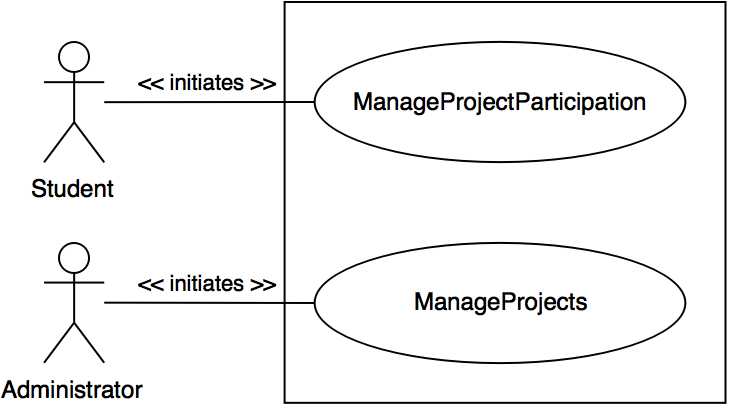
\includegraphics[scale=0.5]{imgs/high-level-use-case.png}
	\caption{High-level Use Case Diagram}
\end{figure}

\begin{figure}[H]
	\centering{}
	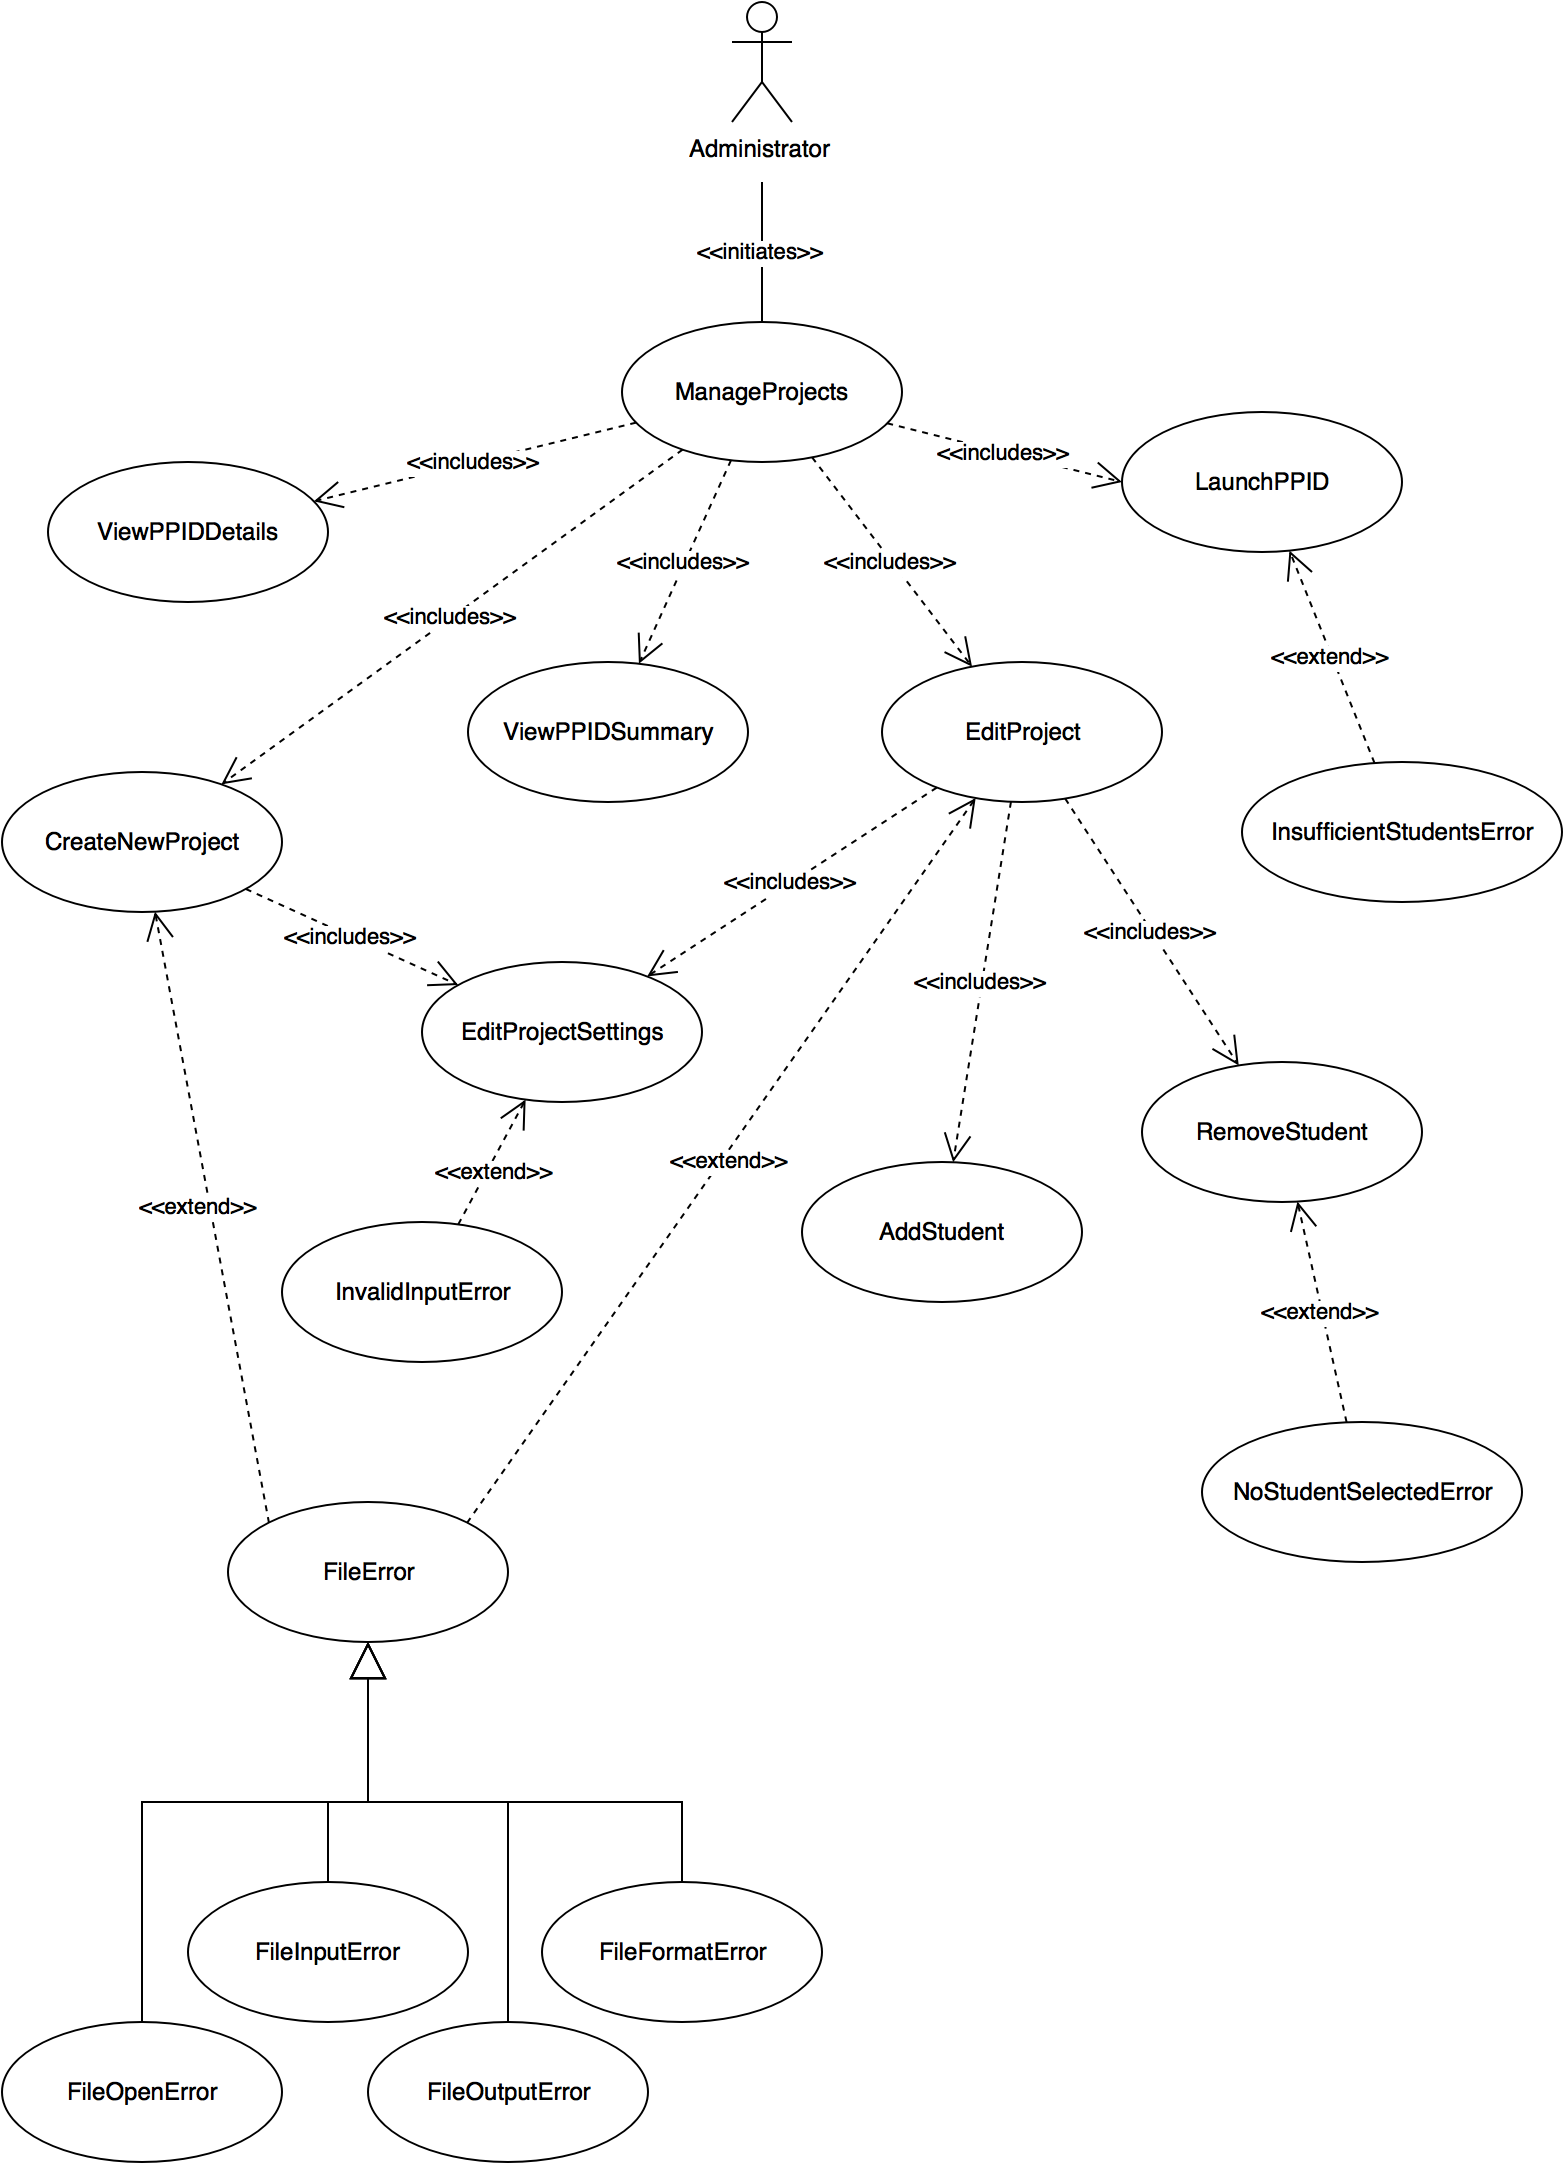
\includegraphics[scale=0.5]{imgs/Administrator-Use-Case.png}
	\caption{Detailed Administrator Use Case Diagram}
\end{figure}

\begin{table}[H]
\caption{High-Level Use Case Descriptions}
\renewcommand{\arraystretch}{1.5}
\everyrow{\hline}
\begin{tabu} to \textwidth {>{\bf}l >{\it}l X}
UC-01 & ManageProjectParticipation & description blah blah \\
UC-02 & Manage Projects & blah \\
\end{tabu}
\end{table}

\begin{table}[H]
\caption{Detailed Use Case Descriptions}
\renewcommand{\arraystretch}{1.5}
\everyrow{\hline}
\begin{tabu} to \textwidth {>{\bf}l >{\it}l X}
UC-03 & CreateNewProject & The Administrator creates a new instance of a project.\\
UC-04 & EditProjectSettings & The Administrator modifies the parameters of a specified project.\\
UC-05 & LaunchPPIDAlgorithm & The Administrator applies the PPID Algorithm to a specified project.\\
UC-06 & CaseThree & blah blah \\
UC-07 & CaseFour & blah \\
UC-08 & SetTeamSize & The Administrator sets team size parameter for the current project.\\
UC-09 & AddStudent & The Administrator adds a Student to the current project.\\
UC-10 & RemoveStudent & The Administrator removes a Student from the current project.\\
UC-11 & SetProjectName & The Administrator sets the project name parameter for the current project.\\
UC-12 & SaveSettings & The Administrator saves the current project's parameters.\\
\end{tabu}
\end{table}

{\renewcommand{\arraystretch}{1.5}
\everyrow{\hline}
\begin{tabu} to \textwidth {>{\it}l X}
\toprule
Use Case Identifier & UC-01 \\
Name & {\bf ManageProjectParticipation} \\
Participating Actors & Student \\
Flow of Events & blah \\
Entry Conditions & \textbullet \hspace{2 mm}blah \\
Exit Conditions & \textbullet \hspace{2 mm}blah \\
Quality Requirements & \textbullet \hspace{2 mm}blah \\
Traceability & \textbullet \hspace{2 mm}blah \\
\toprule
\end{tabu}

\noindent{}
{\renewcommand{\arraystretch}{1.5}
\everyrow{\hline}
\begin{tabu} to \textwidth {>{\it}l X}
\toprule
Use Case Identifier & UC-02 \\
Name & {\bf ManageProjects} \\
Participating Actors & Administrator \\
Flow of Events & 1. The Administrator starts up the Administration process.
2.\\
Entry Conditions & \textbullet \hspace{2 mm}blah \\
Exit Conditions & \textbullet \hspace{2 mm}blah \\
Quality Requirements & \textbullet \hspace{2 mm}blah \\
Traceability & \textbullet \hspace{2 mm}blah \\
\toprule
\end{tabu}

\subsubsection{Object Model}


\subsubsection{Dynamic Model}

\begin{figure}[H]
\protect\caption{Sample 1}


\end{figure}


\begin{figure}[H]
\protect\caption{Sample 2}


\end{figure}

\end{document}
